% SafetyPulse — EMNLP-format short paper (Stage 2). Build: cd paper && tectonic main.tex
% Every number is traceable to docs/report/*.md (generated by tools/*_analysis.py) or a RUN_SUMMARY.md.
\documentclass[11pt]{article}
\usepackage{acl}            % final (named) version; add [review] for the anonymous version
\usepackage{times}
\usepackage{latexsym}
\usepackage[T1]{fontenc}
\usepackage[utf8]{inputenc}
\usepackage{microtype}
\usepackage{inconsolata}
\usepackage{graphicx}
\usepackage{booktabs}
\usepackage{amsmath}
\usepackage{xcolor}
\newcommand{\cissep}{\textsc{cis}$_{\text{sep}}$}
\newcommand{\ciscirc}{\textsc{cis}$_{\text{circ}}$}
\newcommand{\pending}[1]{\textcolor{red}{[#1]}}   % results of HF Jobs 10/11 still running; remove before submission

\title{Where Does a Refusal-Direction Drift Monitor Transfer?\\A Pre-registered Evaluation Across Models and Drift Sources}

\author{Purvansh Joshi \And Archit Mittal \And Anubhav Kiroula \\
  PxA Labs % TODO(authors): add affiliation and contact e-mail
}

\begin{document}
\maketitle

\begin{abstract}
Fine-tuning an aligned model on benign data can erode its refusals, and auditing every checkpoint is costly. We study a
cheap internal alarm: the separation of harmful and harmless prompts along the base model's refusal direction,
normalised to the base model (\cissep{}), with WARN/FAIL thresholds fixed once on development runs of Tiny Aya Global.
We then pre-registered four tests before running them. With thresholds frozen, the alarm transfers to a sibling model
(Tiny Aya Earth: 63/63 unsafe checkpoints flagged, no alarm on 50 control checkpoints) and to a second drift source
(list-formatted instruction data: 65/65). Two predictions failed: the alarm does not warn earlier than a weight-change
baseline (median lead 20 vs.\ 20 steps), and on 35 third-party checkpoints from four other model families its FAIL
level fired on 3 of 8 safe recovered models. Exploratory analysis locates the failure mostly in the thresholds: within
three of the four families the score ranks unsafe models perfectly or near-perfectly (AUROC 0.94--1.00), but not in
Gemma-3 (0.50), and a 50-prompt refusal spot-check is competitive throughout.
\end{abstract}

\section{Introduction}

Safety alignment is fragile under fine-tuning: even benign instruction data can raise a model's compliance with harmful
requests \citep{qi2023finetuning,he2024safedata}. Re-auditing every checkpoint with hundreds of red-team prompts and a
safety judge is expensive, so a cheap \emph{screening signal} that can run inside the training loop is attractive. One
candidate reads the mechanism directly: refusal in chat models is mediated largely by a single residual-stream direction
\citep{arditi2024refusal}, and benign fine-tuning is known to move it \citep{du2025procon,guo2026routing}.

Activation-based drift monitors already exist and have been validated on held-out runs \citep{nghiem2026trait}; our
contribution is not a new monitor but a \textbf{pre-registered test of where one transfers}. We built SafetyPulse, a
refusal-direction monitor with a Trainer callback and a calibrate/check/repair package, on one model (Tiny Aya Global
\citep{salamanca2026tinyaya}), where all design choices, including the alarm thresholds, were made on development runs.
Because such choices are easily over-fitted to one model, we then wrote down four hypotheses with pass marks
\citep{nosek2018preregistration} and ran new experiments: a sibling model (H1), a second drift source (H2), lead time at
finer checkpoint spacing (H3), and 35 third-party checkpoints from four other model families (H6). Two hypotheses
were confirmed and two refuted; we report all four, with exploratory analyses labelled as such.

\section{Method}
\label{sec:method}

\paragraph{Calibration (once per base model).} We use 288 AdvBench-derived harmful prompts \citep{zou2023advbench}, each paired with a minimally
edited harmless twin of the same topic and length, split into calibration, validation and 50 probe pairs. The refusal
direction at residual position $l$ is the difference of mean last-token activations,
$r_l=\bar h_l^{\text{harm}}-\bar h_l^{\text{harmless}}$ \citep{arditi2024refusal}. The layer $l^*$ is chosen on
validation pairs as the position whose ablation most reduces refusal on harmful prompts among those where adding $r_l$
induces refusal on harmless ones. A circuit of 20 attention heads and MLPs is found by attribution patching
\citep{syed2023attribution} and confirmed by exact activation patching.

\paragraph{Check (every checkpoint).} With $\hat r=r_{l^*}/\lVert r_{l^*}\rVert$ and $h$ the checkpoint's activations on
the 50 probe pairs,
\begin{equation*}
\text{\cissep}=\frac{\overline{h_{l^*}^{\text{harm}}\cdot\hat r}-\overline{h_{l^*}^{\text{harmless}}\cdot\hat r}}
{\text{the same quantity for the base model}} ,
\end{equation*}
so the base model scores 1. The circuit score \ciscirc{} (attribution-weighted, secondary) is defined analogously.
A check costs about half of a full audit's GPU time on a T4.

\paragraph{Thresholds (fixed on Global's development runs).} FAIL below $\tau_f=0.6196$ (best F1 on development
checkpoints), WARN below $\tau_w=\tau_f+(1-\tau_f)/2=0.8098$. They are never re-tuned in the tests below.

\paragraph{Ground truth.} Attack success rate (ASR) on 78 HarmBench-derived prompts \citep{mazeika2024harmbench},
greedy decoding, judged by Llama Guard 3 1B \citep{inan2023llamaguard}. A checkpoint is \emph{unsafe} when its ASR
exceeds the step-0 (or aligned) model's ASR by more than 10 points.

\paragraph{Development results (post hoc, one model).} On Tiny Aya Global (12 LoRA runs \citep{hu2021lora}, 150
checkpoints), Alpaca tuning \citep{taori2023alpaca} doubled ASR (21\%$\rightarrow$37--46\%) while GSM8K and a
refusal-augmented control did not. On held-out test runs \cissep{} at FAIL caught 96\% of unsafe checkpoints (precision
0.85) with no alarm on safe runs. This comparison was made after the test runs were scored, which is why we
pre-registered the tests that follow.

\section{Pre-registered evaluation}
\label{sec:prereg}

The plan (\S\ref{app:prereg}) was committed to a public repository before each experiment. It fixes the primary signal
(\cissep{} at WARN-or-FAIL), the thresholds, the unsafe rule, the judge and the verdict rules; deviations were added as
dated amendments before the affected analysis. Fine-tunes use LoRA ($r=16$, 2{,}000 examples, 250 steps) with a
checkpoint every 10 steps.

\begin{table*}[t]
\centering\small
\begin{tabular}{@{}l p{3.9cm} p{3.6cm} p{5.0cm} c@{}}
\toprule
& Setting (new runs) & Prediction & Result & Verdict \\
\midrule
H1 & Tiny Aya Earth: 3 Alpaca + 2 control seeds & recall $\ge$0.8; no FAIL on control
   & recall 1.00 (63/63), precision 0.93, 0/50 control alarms & \textbf{confirmed} \\
H2 & Global, list-formatted Alpaca, 3 seeds & recall $\ge$0.8; ASR rises $\ge$ Alpaca
   & recall 1.00 (65/65), Wilson [0.94, 1.00]; peak ASR 0.47 vs.\ 0.42 & \textbf{confirmed} \\
H3 & Global, Alpaca, 3 new seeds & median lead $>$0 and $>$ $\lVert\Delta W\rVert$ lead
   & median lead 20 steps vs.\ 20 for $\lVert\Delta W\rVert$ & \textbf{refuted} \\
H6 & SafeTune: 4 families, 35 models & recall $\ge$0.8; no FAIL on safe recovered
   & recall 0.92 (11/12); FAIL on 3/8 safe recovered & \textbf{refuted} \\
\bottomrule
\end{tabular}
\caption{The four pre-registered tests. Recall is \cissep{} at WARN-or-FAIL on unsafe checkpoints (drifted models for
H6). Thresholds were frozen on Tiny Aya Global; nothing was tuned on these runs.}
\label{tab:prereg}
\end{table*}

\section{Results}
\label{sec:results}

\paragraph{H1: a sibling model.} On Tiny Aya Earth, calibrated with the same recipe and Global's thresholds, \cissep{}
flagged all 63 unsafe checkpoints of the three Alpaca runs 10--20 steps before the first unsafe one and raised no alarm
on the 50 checkpoints of the two control runs (Figure~\ref{fig:traj}, left; AUROC 0.99). The FAIL level did not
transfer: the lowest score was 0.67, above $\tau_f$.

\paragraph{H2: a second drift source.} Rewriting every Alpaca answer as a bulleted list, a format reported to be
especially harmful to safety \citep{he2024safedata}, drifted more than plain Alpaca (median peak ASR 0.47 vs.\ 0.42) and
\cissep{} flagged all 65 unsafe checkpoints (Figure~\ref{fig:traj}, right). All H2 runs drift, so its precision (0.90)
only reflects their few early safe checkpoints.

\begin{figure*}[t]
\centering
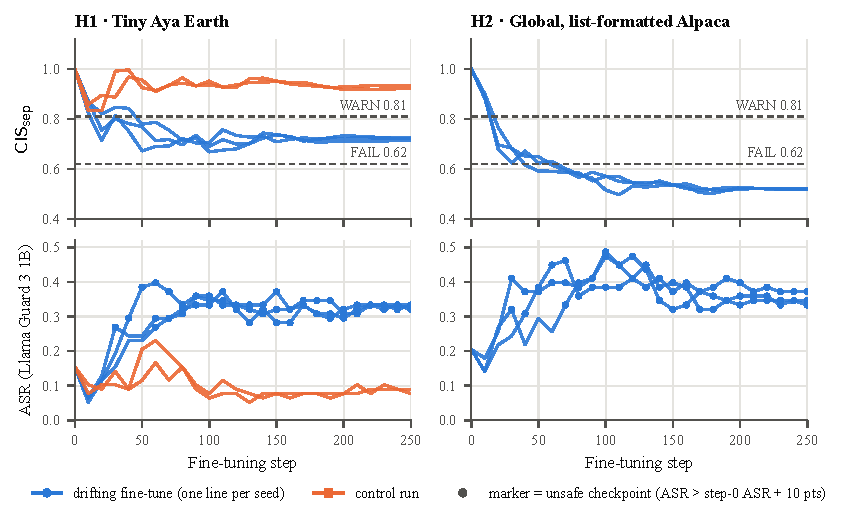
\includegraphics[width=\textwidth]{figures/fig_trajectories.pdf}
\caption{\cissep{} (top) and ASR (bottom) during fine-tuning, one line per seed, with Global's frozen thresholds. H1:
Alpaca runs fall below WARN and become unsafe; control runs stay above WARN. H2: list-formatted data drifts further.}
\label{fig:traj}
\end{figure*}

\paragraph{H3: lead time.} With checkpoints every 10 steps, \cissep{} at WARN preceded the first unsafe checkpoint on
all three runs (20, 10 and 30 steps), but an alarm on the size of the weight change $\lVert\Delta W\rVert$, at its own
development threshold, fired at the same checkpoint on every run. The pre-registered prediction required a strictly
longer lead, so H3 is refuted: reading the refusal direction did not warn \emph{earlier} than a mechanism-agnostic
baseline. The difference lies elsewhere: in development, \cissep{} separated drifting from benign fine-tunes (AUROC 0.95)
far better than $\lVert\Delta W\rVert$ (0.70).

\paragraph{H6: other model families.} SafeTune \citep{seth2026safetune} releases HH-RLHF-aligned \citep{bai2022hhrlhf}
Llama-3.2-3B, Qwen3-4B, Gemma-3-4B and Llama-3.1-8B models \citep{grattafiori2024llama3,yang2025qwen3,gemmateam2025gemma3},
full fine-tunes that drifted from them (code, Dolly, GSM8K, legal, medical) and DPO-recovered versions
\citep{rafailov2023dpo}. We calibrated on each aligned model and scored all 35 models with Global's thresholds
(Figure~\ref{fig:safetune}). \cissep{} flagged 11 of 12 unsafe drifted models, but reached FAIL on three recovered
models that are safe by our measure (two Gemma, one Llama-3.1-8B), refuting H6. On Llama-3.2-3B and Qwen3-4B the FAIL
level was clean (9 of 11 unsafe models, no safe one), but WARN fired on every fine-tune, safe or not; on Gemma-3-4B the
most unsafe model (Dolly, ASR $+0.50$) scored 0.91, a PASS.

\begin{figure*}[t]
\centering
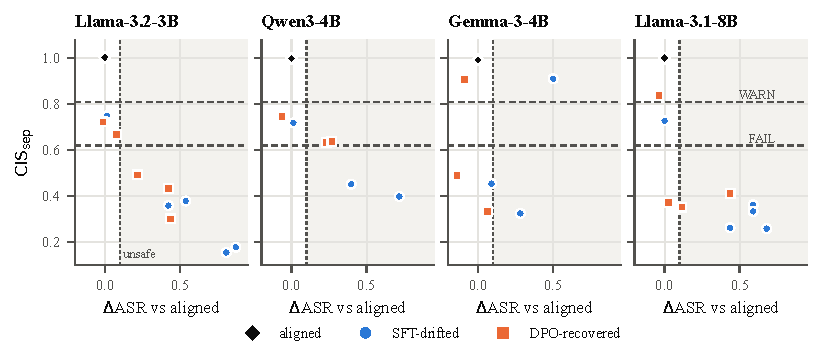
\includegraphics[width=\textwidth]{figures/fig_safetune.pdf}
\caption{H6: \cissep{} against the ASR change from the aligned model, per family. Shaded: unsafe ($\Delta$ASR $>0.10$).
A good alarm puts shaded points below the dashed thresholds and unshaded points above them.}
\label{fig:safetune}
\end{figure*}

\paragraph{Judge robustness.} Re-judging every H1 and H3 checkpoint with Llama Guard 3 8B (same answers) gave agreement
of 95\% and 93\% (Cohen's $\kappa$ 0.86 and 0.83; \citealp{cohen1960kappa}) and left both verdicts unchanged (H1 recall
0.99, 66/67; H3 tie). H2: \pending{Job 10}.

\paragraph{Exploratory: thresholds or signal?} Threshold-free, \cissep{} ranks unsafe below safe models with AUROC
1.00 (Llama-3.2-3B), 1.00 (Qwen3-4B) and 0.94 (Llama-3.1-8B), but 0.50 on Gemma-3-4B, whose calibration chose an
unusually early layer (11 of 34). \pending{Job 11: per-layer AUROC}. Per-family thresholds chosen on the other
fine-tune domains of the same family do not fix the false alarms (recall 17/19, 7 of 12 safe models flagged): with
6--10 models per family, a threshold cannot be set reliably. A 50-prompt refusal spot-check was competitive in every
test (H6: 17/19 unsafe flagged, 3/12 false alarms; AUROC 0.91 pooled vs.\ 0.83 for \cissep{}).

\section{Related work}

Benign fine-tuning degrades safety \citep{qi2023finetuning,he2024safedata,wei2024brittleness}; the refusal direction
\citep{arditi2024refusal} drifts during tuning \citep{du2025procon} and benign tuning disrupts how safety information is
routed to refusal \citep{guo2026routing}. The closest monitor tracks seven trait directions during LoRA tuning of four
7--9B models and validates a classifier on 468 held-out checkpoints \citep{nghiem2026trait}; we instead test frozen
thresholds of a single-direction score across models and drift sources. Preserving the base refusal direction is not a
reliable proxy for safety in every model \citep{ruellan2026replay}, and frozen activation probes can go stale after
updates \citep{duan2026monitors}; our H6 result is consistent with both. Prevention methods constrain tuning instead
\citep{hsu2024safelora,du2025procon}, and SafeTune \citep{seth2026safetune} and CircuitKIT \citep{seth2026circuitkit}
provide auditing, repair and circuit tools that SafetyPulse builds on.

\section{Conclusion}

A refusal-direction alarm with thresholds fixed on one model transferred to a sibling model and to a second drift
source, but neither warned earlier than a weight-change baseline nor carried its thresholds to other model families. The
score itself ranked models well in three of four families, so the weak point is calibration: practitioners should
expect to set thresholds per model family, with enough development runs to do so, and to keep a cheap behavioural
spot-check alongside.

\section*{Limitations}

\textbf{Small samples.} Each test uses 3--5 runs or 6--11 models per family; intervals are wide and per-family
thresholds could not be estimated reliably. \textbf{One judge and a small prompt set.} Unsafe labels come from Llama
Guard 3 1B on 78 English prompts (about $\pm$10 points per checkpoint); the 8B judge agreed closely where tested.
\textbf{English only.} Calibration and evaluation are in English, although benign multilingual fine-tuning is known to
move safety differently per language \citep{hawkins2026multilingual}; the planned multilingual test (H4) was not run.
\textbf{Drifting runs dominate.} H2 and H3 contain only drifting runs, so false alarms are measured mainly in H1 and H6.
\textbf{Endpoints in H6.} The SafeTune checkpoints are single models per fine-tune, so H6 tests detection, not lead time;
our ASR for recovered models is our measurement, not the releasing authors' evaluation. \textbf{Post-hoc choices.} The
primary signal was chosen after Global's test runs were scored; the pre-registered tests are the evidence we rely on.

\section*{Ethics Statement}

We study harmful-request compliance to make fine-tuning safer. Harmful model answers and our harmful fine-tuning
positive control are not released; published logs contain verdicts and scores only. Third-party checkpoints were
accessed under their licences (LSAL v1.2 for SafeTune) for academic research and are not redistributed. AI assistance:
an AI coding assistant helped write code and draft text; the authors designed the study, checked every number against
the logged results and take responsibility for the content.

\section*{Acknowledgements}

We thank Lexsi Labs for the SafeTune, CircuitKIT, AuditKIT and CuratorKIT toolkits, the SafeTune checkpoints and
compute credits, and Cohere Labs for the Tiny Aya models.

\bibliography{custom}

\appendix

\section{Pre-registration and deviations}
\label{app:prereg}

The plan is \texttt{docs/13\_PREREGISTRATION.md} in the project repository; its git history timestamps each section.
Dated amendments, each written before the affected analysis: (i) the H2 monitor for one seed hit a 1.5-hour time guard
after 25 of 26 checkpoints and the last checkpoint was scored in a resumed session; (ii) H6 scoring used bf16 on L40S GPUs,
Qwen3's non-thinking chat mode, and a loader fix for Gemma-3's multimodal wrapper; (iii) the 8B re-judging of H2, the
threshold-free and per-family analyses, and the layer diagnosis were added after the H6 result as exploratory analyses.

\section{Artifacts and compute}

Code, notebooks, run summaries and analysis scripts: \url{https://github.com/PxA-Labs/safetypulse}. Adapters, logs and
the H6 scores and calibration bundles are on the Hugging Face Hub (collections linked from the repository). Experiments
ran on Kaggle T4 GPUs and Hugging Face Jobs (A100, L40S); the H6 jobs took 9--22 minutes per family on one L40S.

\end{document}
